\chapter{Dasar Teori}
\label{chap:dasar_teori}
Pada bab ini akan dijelaskan dasar-dasar teori mengenai Android SDK, Google VR SDK,Kuaternion, \textit{Sensor Fusion}, dan algoritme \textit{Head Motion Detection}.

% 2.1 Android SDK
\section{Android SDK}
\label{sec:android_sdk}

Android SDK(\textit{software development kit}) adalah kumpulan \textit{source code, development tools, emulator,} dan semua \textit{libraries} untuk membuat suatu aplikasi untuk \textit{platform} Android.\cite{developers2011android} IDE (\textit{integrated development environment}) yang resmi untuk Android SDK adalah Android Studio. Android Studio dapat di download di halaman situs Google Developer,\footnote{https://developer.android.com/studio/archive.html} sekaligus dengan Android SDKnya.  

% 2.1.1 Struktur File Android Studio Project
\subsection{Struktur File Android Studio Project}

				Pada saat membuat \textit{project} baru, Android Studio akan membuatkan \textit{folder-folder} standar secara otomatis. \textit{Folder-folder} tersebut akan memiliki tujuannya masing-masing. Penjelasan \textit{folder-folder} tersebut akan dijelaskan pada Gambar  \ref{fig:android-studio-structure}.
				\begin{figure}[htbp]
				\dirtree{%
					.1 {module}.
					.2 {build} \ldots{} \begin{minipage}[t]{5cm}Folder yang mengandung file-file dari hasil pembangunan \textit{project}{.}\end{minipage}.
					.2 {libs} \ldots{} \begin{minipage}[t]{5cm}Folder yang mengandung \textit{libraries} privat{.}\end{minipage}.
					.2 {src} \ldots{} \begin{minipage}[t]{5cm}Folder yang mengandung semua kode dan file sumber untuk suatu modul{.}\end{minipage}.
					.3 {androidTest} \ldots{} \begin{minipage}[t]{5cm}Folder yang mengandung kode untuk mengetes yang berjalan di perangkat Android{.}\end{minipage}.
					.3 {main} \ldots{} \begin{minipage}[t]{5cm}Folder yang mengandung file-file kode dan file sumber inti dari suatu module{.}\end{minipage}.
					.4 {AndroidManifest.xml} \ldots{} \begin{minipage}[t]{5cm}File yang mendeskripsikan sifat dari aplikasi dan setiap komponennya{.}\end{minipage}.
					.4 {java} \ldots{} \begin{minipage}[t]{5cm}Folder yang mengandung kode-kode java{.}\end{minipage}.
					.4 {jni} \ldots{} \begin{minipage}[t]{5cm}Folder yang mengandung kode-kode yang menggunakan Java Native Interface (JNI){.}\end{minipage}.
					.4 {gen} \ldots{} \begin{minipage}[t]{5cm}Folder yang mengandung file-file java yang dihasilkan oleh Android Studio{.}\end{minipage}.
					.4 {res} \ldots{} \begin{minipage}[t]{5cm}Folder yang mengandung file-file sumber untuk aplikasi, seperti file drawable, layout, dan UI String{.}\end{minipage}.
					.4 {assets} \ldots{} \begin{minipage}[t]{5cm}Folder yang mengandung aset-aset untuk pembuatan aplikasi seperti texture dan data{.}\end{minipage}.
					.2 {build.gradle} \ldots{} \begin{minipage}[t]{5cm}File yang mendefinisikan konfigurasi modul untuk proses build{.}\end{minipage}.
					.1 {build.gradle} \ldots{} \begin{minipage}[t]{5cm}File yang mendefinisikan konfigurasi proses build untuk project yang berlaku untuk semua modul{.}\end{minipage}.
				}
				\caption{Tampilan struktur folder pada \textit{project} Android Studio}
				\label{fig:android-studio-structure}
				\end{figure}
% 2.1.2 Membuat User Interface
\subsection{Membuat User Interface}

Pada subbab ini akan dijelaskan bagaimana membuat \textit{layout} di XML termasuk \textit{text field} dan \textit{button}\cite{android_developers}

% Sub 2.1.2 Hierarki (GUI) untuk Aplikasi Android
\subsubsection{Hierarki \textit{Graphical User Interface} (GUI) untuk Aplikasi Android}
\label{sssec:hierarki_gui_untuk_aplikasi_android}
GUI untuk aplikasi Android dibuat dengan hierarki dari objek View dan ViewGroup (Gambar \ref{fig:viewgroup}). Objek-objek dari View biasanya adalah \textit{UI (User Interface) Widgets} seperti Button atau TextField. Objek-objek dari ViewGroup tidak terlihat oleh \textit{view containers} yang mendefinisikan bagaimana \textit{child views} ditata seperti \textit{grid} atau \textit{vertical list}.

\begin{figure}[htbp]
	\centering
		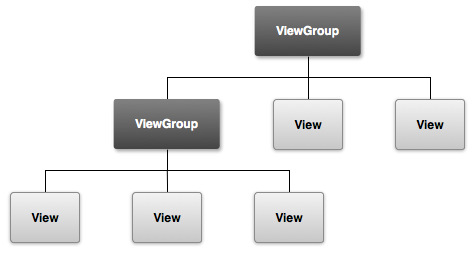
\includegraphics[scale=1]{Gambar/viewgroup.png}
	\caption{Ilustrasi bagaimana percabangan objek ViewGroup pada \textit{layout} dan mengandung objek View lainnya.}
	\label{fig:viewgroup}
\end{figure}

Android menggunakan \textit{file} XML yang berkorespondesi kepada \textit{subclasses} dari View dan ViewGroup, sehingga UI dapat buat dalam XML menggunakan hierarki dari elemen UI.

\subsubsection{Atribut-atribut Objek View}
\label{sssec:atribut_atribut_objek_view}
Pada subbab ini akan dijelaskan atribut-atribut object View yang digunakan dalam membuat GUI pada file activity\_main.xml
\begin{itemize}
	\item \textbf{android:id}
	Atribut ini merupakan identifikasi dari suatu view. Atribut ini dapat digunakan untuk menjadi referensi \textit{object} dari kode aplikasi seperti membaca dan manipulasi objek tersebut (Akan dijelaskan lebih lanjut pada subbab \ref{sec:activity}). Tanda '@' dibutuhkan ketika melakukan referensi object dari suatu XML. Tanda '@' tersebut diikuti dengan tipe (id pada kasus ini), \textit{slash}, dan nama (edit\_message pada Listing \ref{lst:atribute-view}). Tanda tambah (+) sebelum tipe hanya dibutuhkan jika ingin mendefinisikan \textit{resource ID} untuk pertama kalinya.
	\item \textbf{android:layout\_width} dan \textbf{android:layout\_height}
	Atribut ini digunakan untuk mendefinisikan panjang dan lebar dari suatu objek View. Daripada menggunakan besar yang spesifik untuk panjang dan lebarnya, lebih baik menggunakan "wrap\_content". Nilai "wrap\_content" ini akan memberikan spesifikasi viewnya hanya akan sebesar yang dibutuhkan untuk memuat seluruh isi dari View. Jika menggunakan "match\_parent" pada kasus Listing \ref{lst:atribute-view} View akan memenuhi layar, karena besarnya akan mengikuti besar dari \textit{parent}-nya LinearLayout.

	\item \textbf{android:hint}
	Atribut ini merupakan \textit{default string} untuk di tampilkan ketika objek View kosong. Daripada menggunakan \textit{hard-coded string} sebagai \textit{nilai} untuk ditampilkan, nilai "@string/edit\_message" mengacu ke sumber string pada \textit{file} yang berbeda. Karena mengacu ke sumber konkret, maka tidak dibutuhkan tanda tambah (+). Nilai string ini akan di simpan pada file Strings.xml yang ditunjukkan pada Listing \ref{lst:string-xml}.
	\begin{lstlisting}[caption={Contoh kode pada string.xml},label={lst:string-xml},language=xml]
	<resources>
    <string name="app_name">MyFirstAndroidApp</string>
    <string name="edit_message">Ini adalah hint</string>
    <string name="button_send">Send</string>
	</resources>

\end{lstlisting}


	\item \textbf{android:onClick}
	Atribut ini akan memberitahu sistem untuk memanggil \textit{method} yang sesuai namanya (contoh pada Listing \ref{lst:atribute-view} adalah \textbf{sendMessage()}) di Activity ketika pengguna melakukan klik pada \textit{button} tersebut. Agar \textit{system} dapat memanggil \textit{method} yang tepat, \textit{method} tersebut harus memenuhi kriteria berikut.
	\begin{itemize}
		\item \textit{Access Modifier} haruslah \textit{public}.
		\item Harus \textit{void return value}nya.
		\item Mempunyai View sebagai parameter satu-satunya. View ini akan diisi dengan View yang di klik.
	\end{itemize}
\begin{lstlisting}[caption={Contoh kode file XML pada folder layout},label={lst:atribute-view},language=xml]
	<LinearLayout
		xmlns:android="http://schemas.android.com/apk/res/android"
		xmlns:tools="http://schemas.android.com/tools"
		android:layout_width="match_parent"
		android:layout_height="match_parent"
		android:orientation="horizontal">
		<EditText android:id="@+id/edit_message"
				android:layout_weight="1"
				android:layout_width="0dp"
				android:layout_height="wrap_content"
				android:hint="@string/edit_message" />
		<Button
				android:layout_width="wrap_content"
				android:layout_height="wrap_content"
				android:text="@string/button_send"
				android:onClick="sendMessage" />
	</LinearLayout>
\end{lstlisting}
\end{itemize}


\subsection{Activity}
\label{sec:activity}
Activity adalah suatu hal yang fokus pada apa yang bisa pengguna lakukan.
\cite{android_developers} Hampir semua Activity berinteraksi dengan pengguna, jadi kelas Activity akan membuat suatu halaman baru yang bisa ditambahkan dengan View. Selain dapat ditampilkan kepada pengguna dengan halaman \textit{full-screen}, Activity juga dapat ditampilkan dengan cara lain: seperti halaman \textit{floating} atau tertanam di Activity lain.

\subsubsection{Activity Lifecycle}
\label{sssec:activity_lifecycle}
\begin{figure}[htbp]
	\centering
		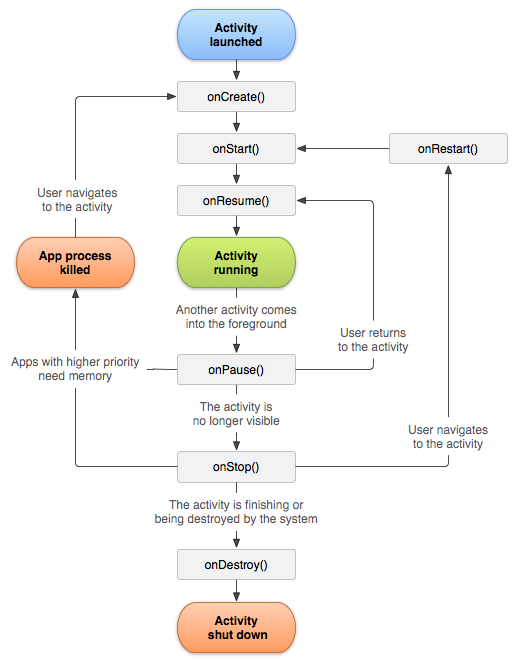
\includegraphics[scale=0.48]{Gambar/activity-lifecycle.png}
	\caption{\textit{State diagram} siklus Activity}
	\label{fig:activity-lifecycle}
\end{figure}

Aktivitas dalam sistem android di atur sebagai \textit{activity stack}. Ketika ada Activity baru yang dimulai, Activity tersebut ditempatkan di paling atas pada \textit{stack} dan menjadi Activity aktif. Activity sebelumnya akan tetap berada di bawah stack, dan tidak akan muncul lagi sampai Activity yang baru berakhir. 

Activity didasari dari empat kondisi:
\begin{itemize}
	\item Jika Activity berada di latar depan pada layar, Activity tersebut sedang aktif.
	\item Jika Activity sudah tidak menjadi fokus tetapi masih dapat terlihat, Activity tersebut sedang berhenti sementara. Pada kondisi ini Activity tersebut masih berjalan, tapi bisa diberhentikan ketika sistem berada dalam situasi kekurangan memori.
	\item Jika suatu Activity benar-benar dihalangi oleh Activity lain, Activity tersebut telah berhenti. Activity tersebut akan tetap mengingat seluruh keadaan dan informasi anggota tetapi, Activity tersebut tidak lagi terlihat oleh pengguna jadi tampilan halamannya akan tersembunyi dan seringkali akan diberhentikan Activity-nya ketika sistem membutuhkan memori.
	\item Jika suatu Activity sedang berhenti sementara atau berhenti total, sistem dapat membuang Activity dari memori dengan cara menanyakan kepada pengguna untuk menghentikannya atau langsung diberhentikan oleh sistem. Jika Activity tersebut ditampilkan lagi kepada pengguna, Activity tersebut harus memulai dari awal dan kembali ke keadaan sebelumnya.
\end{itemize}
Gambar \ref{fig:activity-lifecycle} menunjukkan pentingnya alur keadaan dari suatu Activity. Gambar segi empat menggambarkan \textit{callback \textit{method}s} yang dapat ditambahkan suatu implementasi untuk melakukan operasi ketika Activity berubah kondisi. Oval berwarna merupakan kondisi-kondisi utama dari suatu Activity.
Ada 3 \textit{key loops} untuk memantau suatu Activity:
\begin{itemize}
	\item \textit{Entire lifetime} terjadi diantara pemanggilan pertama pada onCreate(Bundle) sampai ke suatu pemanggilan terakhir onDestroy(). Suatu Activity akan melakukan semua persiapan pada kondisi umum pada \textit{method} onCreate(), dan melepaskan seluruh sisa pemrosesan pada \textit{method} onDestroy().
	\item \textit{Visible lifetime} terjadi antara pemanggilan onStart() sampai pemanggilan yang sesuai pada onStop(). Pada tahap ini pengguna dapat melihat Activity pada layar meski pun tidak berada pada \textit{foreground} dan berinteraksi dengan pengguna.
	\item \textit{Foreground lifetime} terjadi antara pemanggilan \textit{method} onResume() sampai ke satu pemanggilan akhir onDestroy(). Pada tahap ini Activity berada di depan semua Activity lainnya dan sedang berinteraksi dengan pengguna.
\end{itemize}


\subsection{Android Sensor Framework}
\label{sec:android_sensor_framework}
Sebagian besar dari perangkat android sudah memiliki sensor yang mengukur gerakan, orientasi, dan berbagai keadaan lingkungan.\cite{android_developers} Sensor-sensor ini dapat memberikan data mentah dengan tingkat akurasi yang tinggi. Sensor ini juga berguna untuk memantau pergerakan tiga dimensi atau posisi perangkat. Sensor ini juga dapat memantau perubahan keadaan lingkungan yang dekat dengan perangkat. 
Android mendukung tiga kategori sensor:
\begin{itemize}
	\item \textbf{Sensor gerak}
	Sensor-sensor ini mengukur akselerasi dan rotasi pada tiga sumbu. Kategori sensor ini meliputi \textit{accelerometer}, sensor gravitasi, \textit{gyroscope}, dan \textit{rotation vector}. 
	\item \textbf{Sensor keadaan lingkungan}
	Sensor-sensor ini mengukur berbagai keadaan lingkungan seperti suhu udara, tekanan, pencahayaan, dan kelembapan. Kategori sensor ini termasuk barimeter, fotometer dan termometer.
	\item \textbf{Sensor posisi}
	Sensor-sensor ini mengukur posisi perangkat. Kategori sensor ini meliputi sensor orientasi dan magnetometer.
\end{itemize}
Android Sensor Framework membantu \textit{developers} untuk mengakses berbagai jenis sensor. Beberapa sensor berbasis perangkat keras dan beberapa sensor berbasis perangkat lunak. Sensor berbasis perangkat keras mendapatkan data dengan langsung mengukur sifat lingkungan tertentu, seperti percepatan, kekuatan medan geomagnetik, atau perubahan sudut. Sensor berbasis perangkat lunak mendapatkan data dari satu atau lebih sensor berbasis perangkat keras. Sensor berbasis perangkat lunak ini juga terkadang disebut sensor virtual atau sensor sintetis. Pada tabel berikut akan dirincikan tipe-tipe setiap sensor posisi dan gerak, deskripsi, dan penggunaan umumnya.

\begin{table}[htbp]
	\centering
	\caption{Tipe-tipe Sensor pada Android}
\begin{tabular}{|p{6.3cm}| p{1.5cm}| p{5cm}| p{2.4cm}|} 
\hline
Sensor & Tipe & Deskripsi & Penggunaan umum\\ \hline
TYPE\_ACCELEROMETER & Perangkat Keras & Mengukur percepatan dalam \(m/s^2\) yang terjadi pada perangkat di semua tiga sumbu fisik (x,y,z), termasuk percepatan gravitasi. & Deteksi gerak(goncangan, keseimbangan, dan lain-lain)\\ \hline
TYPE\_GRAVITY & Perangkat Lunak atau Perangkat Keras & Mengukur percepatan gravitasi dalam \(m/s^2\) yang terjadi pada perangkat di tiga sumbu fisik (x,y, dan z) & Deteksi gerak(goncangan, keseimbangan, dan lain-lain)\\ \hline
TYPE\_GYROSCOPE & Perangkat Keras & Mengukur rata-rata rotasi sudut dalam \(rad/s\) di tiga sumbu fisik (x,y, dan z). & Deteksi rotasi (putaran, belokan, dan lain-lain).\\ \hline
TYPE\_LINEAR\_ACCELERATION & Perangkat Lunak atau Perangkat Keras & Mengukur percepatan dalam \(m/s^2\) yang terjadi pada perangkat di semua tiga sumbu fisik (x,y,z), tidak termasuk percepatan gravitasi. & Memantau percepatan pada suatu sumbu.\\ \hline
TYPE\_MAGNETIC\_FIELD & Perangkat Keras & Mengukur medan magnet sekitar untuk semua tiga sumbu fisik (x,y, dan z) di satuan \(\mu T\). & Membuat Kompas.\\ \hline
TYPE\_ORIENTATION & Perangkat Lunak & Mengukur derajat rotasi yang terjadi pada perangkat pada semua tiga sumbu fisik (x,y, dan z). & Menentukan posisi perangkat \\ \hline
TYPE\_ROTATION\_VECTOR & Perangkat Lunak dan Perangkat Keras & Mengukur orientasi dari suatu perangkat dengan menyediakan tiga elemen dari vektor rotasi perangkat. & Deteksi gerak dan deteksi rotasi.\\ \hline
\end{tabular}
\end{table}
\subsubsection{Sistem Koordinat Sensor}
\label{sssec:sistem_koordinat_sensor}
Pada umumnya, sensor framework menggunakan sistem tiga sumbu koordinat standar untuk mengekspresikan nilai data. Sebagian besar sensor sistem koordinat akan relatif terhadap layar perangkat bila perangkat dibuat dalam orientasi standar (lihat Gambar \ref{fig:axis-device})
\begin{figure}[htbp]
	\centering
		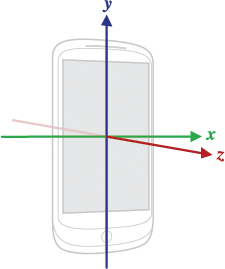
\includegraphics[scale=1]{Gambar/axis-device.png}
	\caption{Sistem koordinat (relatif dengan perangkatnya) yang digunakan oleh Sensor API}
	\label{fig:axis-device}
\end{figure}
Sensor-sensor yang menggunakan sistem tiga sumbu seperti Gambar \ref{fig:axis-device} adalah sebagai berikut :
\begin{itemize}
	\item Accelerometer
	\item Sensor Gravitasi
	\item Gyroscope
	\item Sensor Percepatan Linear
	\item Sensor Medan Geomagnetik
\end{itemize}
Koordinat sistem yang sumbu-nya tidak tertukar ketika orientasi perangkat berubah. Sistem koordinat sensor tidak pernah berubah seiring perangkatnya bergerak. Dalam aplikasi Android tidak dapat diberikan asumsi bahwa standar orientasi perangkat Android adalah \textit{portrait}. Kebanyakan perangkat \textit{Tablet} standar orientasi-nya adalah \textit{landscape}. Sistem koordinat sensor selalu di dasarkan pada orientasi dasar dari suatu perangkat Android.
\subsubsection{Mengidentifikasi Sensor dan Kemampuan Sensor}
\label{sssec:mengidentifikasi_sensor_dan_kapabilitas_sensor}
Android Sensor Framework menyediakan beberapa \textit{method} yang dapat membuat developer mudah untuk menentukan sensor mana yang akan digunakan. API-nya juga dapat menyediakan \textit{method} yang memungkinkan penggunanya menentukan kemampuan masing-masing sensor, seperti jangkauan maksimum, resolusi, dan kebutuhan dayanya.
Untuk mengidentifikasi sensor-sensor yang ada pada perangkat, hal pertama yang perlu dilakukan adalah mendapatkan referensi sensor tersebut. Untuk mendapatkan referensi tersebut, dapat dilakukan dengan membuat instansi dari kelas SensorManager dan memanggul \textit{method} getSystemService() dan memasukkan isi parameter-nya dengan SENSOR\_SERVICE. Contohnya pada Listing \ref{lst:init-sensor-manager}.
 
\begin{lstlisting}[caption={Contoh inisialisasi kelas SensorManager},label={lst:init-sensor-manager},language=java]
private SensorManager mSensorManager;
...
mSensorManager = (SensorManager) getSystemService(Context.SENSOR_SERVICE);
\end{lstlisting}

Kemudian untuk mendapatkan daftar dari setiap sensor pada suatu perangkat dapat dilakukan dengan cara memanggil \textit{method} getSensorList() dan menggunakan konstanta TYPE\_ALL pada kelas Sensor. Contohnya pada Listing \ref{lst:get-sensor-lists}

\begin{lstlisting}[caption={Contoh untuk mendapatkan daftar dari setiap sensor yang ada},label={lst:get-sensor-lists},language=java]
List<Sensor> deviceSensors = mSensorManager.getSensorList(Sensor.TYPE_ALL);
\end{lstlisting}

Namun jika ingin mendapatkan sensor-sensor yang sesuai dengan tipe sensor yang diberikan, dapat menggunakan TYPE\_GYROSCOPE, TYPE\_LINEAR\_ACCELERATION, TYPE\_GRAVITY, atau TYPE\_GRAVITY.

Untuk menentukan jenis tertentu dari sensor yang ada pada perangkat dapat didapatkan dengan \textit{method} getDefaultSensor() dengan dimasukkan dengan konstanta yang berada pada kelas Sensor. Jika perangkatnya memiliki lebih dari satu sensor dari tipe sensor yang diberikan, salah satu dari sensor tersebut akan dianggap sebagai sensor dasar. Jika sensor dasarnya tidak ada untuk sensor tersebut, perangkat tersebut berarti tidak memiliki sensor dengan jenis yang diberikan. Listing \ref{lst:check-sensor} adalah contoh untuk mengecek apakah perangkat yang digunakan memiliki sensor dengan jenis yang diberikan.

\begin{lstlisting}[caption={Contoh untuk mengecek apakah perangkat yang digunakan memiliki sensor dengan jenis yang diberikan},label={lst:check-sensor},language=java]
private SensorManager mSensorManager;
...
mSensorManager = (SensorManager) getSystemService(Context.SENSOR_SERVICE);
if (mSensorManager.getDefaultSensor(Sensor.TYPE_MAGNETIC_FIELD) != null){
  // Sukses! Perangkat ini memiliki sensor magnetometer.
  }
else {
  // Gagal! Perangkat ini tidak memiliki sensor magnetometer.
  }
\end{lstlisting}

Jika ingin membatasi versi atau vendor dari sensor yang akan digunakan, dapat menggunakan \textit{method} getVendor() dan getVersion(). Seperti pada Listing \ref{lst:check-sensor-version} yang mengharuskan sensor gravitasi ber-\textit{vendor} "Google Inc." dan memiliki versi 3. Jika sensor tersebut tidak tersedia pada perangkat, sensor accelerometer yang digunakan.

\begin{lstlisting}[caption={Contoh untuk mengecek apakah perangkat yang digunakan memiliki sensor dengan jenis yang diberikan},label={lst:check-sensor-version},language=java]
private SensorManager mSensorManager;
private Sensor mSensor;

...

mSensorManager = (SensorManager) getSystemService(Context.SENSOR_SERVICE);
mSensor = null;

if (mSensorManager.getDefaultSensor(Sensor.TYPE_GRAVITY) != null){
  List<Sensor> gravSensors = mSensorManager.getSensorList(Sensor.TYPE_GRAVITY);
  for(int i=0; i<gravSensors.size(); i++) {
    if ((gravSensors.get(i).getVendor().contains("Google Inc.")) &&
       (gravSensors.get(i).getVersion() == 3)){
      // menggunakan sensor gravitasi versi 3.
      mSensor = gravSensors.get(i);
    }
  }
}
if (mSensor == null){
  // Use the accelerometer.
  if (mSensorManager.getDefaultSensor(Sensor.TYPE_ACCELEROMETER) != null){
    mSensor = mSensorManager.getDefaultSensor(Sensor.TYPE_ACCELEROMETER);
  }
  else{
    // Tidak ada sensor gravitasi dan sensor accelerometer!
  }
}
\end{lstlisting}

Salah satu \textit{method} yang sangat berguna lagi adalah, getMinDelay(). Method ini digunakan untuk mengetahui minimum interval waktu suatu sensor dapat menerima data dalam mikro detik. Jika \textit{method} getMinDelay() mengembalikan nilai nol, hal ini berarti sensor ini akan mengembalikan data setiap kali ada perubahan nilai pada sensor tersebut. 

\subsubsection{Memonitor Nilai Sensor}
\label{sssec:memonitor_nilai_sensor}

Untuk memonitor data mentah dari sensor, dibutuhkan untuk melakukan implementasi dua buah \textit{method callback} yang berada pada interface SensorEventListener. Kedua \textit{method} tersebut adalah onAccuracyChanged(Sensor sensor, int accuracy) dan onSensorChanged(SensorEvent event). Sistem android akan memanggil kedua \textit{method} ini ketika terjadi salah satu kondisi ini:

\begin{itemize}
	\item \textbf{Perubahan akurasi sensor.}\\
Dalam kasus ini sistem memanggil \textit{method} onAccuracyChanged(Sensor sensor, int accuracy). Parameter sensor akan diberikan objek Sensor yang telah berubah akurasi-nya, dan parameter accuracy adalah nilai akurasi sensor yang baru.
	\item \textbf{Sensor memberitahu adanya nilai baru.}\\
Dalam kasus ini sistem memanggil \textit{method} onSensorChanged(SensorEvent event), dengan parameter event akan diisi dengan objek SensorEvent untuk mendapatkan nilai barunya. Objek SensorEvent Mengandung semua informasi tentang data sensor yang baru, termasuk: akurasi dari data, sensor yang mendapatkan data, dan catatan waktu data tersebut didapatkan, dan data yang baru yang telah didapatkan.
\end{itemize}

Pada Listing \ref{lst:monitoring-light-sensor} akan ditunjukkan bagaimana menggunakan \textit{method} onSensorChanged(SensorEvent event) untuk memonitor data dari sensor cahaya. Pada Listing \ref{lst:monitoring-light-sensor} akan menampilkan data mentah dari sensor ke TextView yang telah dibuat pada file main.xml sebagai sensor\_data.
\begin{lstlisting}[caption={Contoh memonitor data mentah pada sensor cahaya},label={lst:monitoring-light-sensor},language=java]
public class SensorActivity extends Activity implements SensorEventListener {
  private SensorManager mSensorManager;
  private Sensor mLight;
  private TextView textView;

  @Override
  public final void onCreate(Bundle savedInstanceState) {
    super.onCreate(savedInstanceState);
    setContentView(R.layout.main);

    mSensorManager = (SensorManager) getSystemService(Context.SENSOR_SERVICE);
    mLight = mSensorManager.getDefaultSensor(Sensor.TYPE_LIGHT);
  }

  @Override
  public final void onAccuracyChanged(Sensor sensor, int accuracy) {
    // Hal yang perlu dilakukan aplikasi ketika akurasinya berubah.
  }

  @Override
  public final void onSensorChanged(SensorEvent event) {
    // Sensor cahaya akan mengembalikan 1 nilai saja.
    // Banyak sensor lain yang akan mengembalikan lebih dari 1 nilai.
    float lux = event.values[0];
    // Hal yang perlu dilakukan ketika ada perubahan data.
  }

  @Override
  protected void onResume() {
    super.onResume();
    mSensorManager.registerListener(this, mLight, SensorManager.SENSOR_DELAY_NORMAL);
  }

  @Override
  protected void onPause() {
    super.onPause();
    mSensorManager.unregisterListener(this);
  }
}
\end{lstlisting}
Pada \textit{method} onSensorChanged(SensorEvent event), struktur nilai-nilai yang dikembalikan akan dijelaskan pada subbab \ref{sssec:struktur_nilai_yang_dikembalikan_oleh_sensor}. Pada \textit{method} onResume(), ada pemanggilan \textit{method} registerListener(). Method registerListener() ini berguna untuk menetapkan waktu \textit{delay} pada pemanggilan onSensorChanged(). Untuk menetapkan \textit{delay}-nya dapat menggunakan konstanta yang ada pada kelas SensorManager. Konstanta-konstanta tersebut adalah SENSOR\_DELAY\_NORMAL (200.000 mikro detik),SENSOR\_DELAY\_GAME (20.000 mikro detik),SENSOR\_DELAY\_UI (60.000 mikro detik), atau SENSOR\_DELAY\_FASTEST (0 mikro detik). Pengaturan dasar untuk waktu \textit{delay} ini menggunakan konstanta SENSOR\_DELAY\_NORMAL.
Perlu diperhatikan juga pemesanan sensor ketika activity sedang dihentikan sementara maupun dilanjutkan kembali. Sistem tidak boleh tetap merekam sensor ketika activity tidak aktif. Hal ini diperlukan karena pada saat perangkat android menggunakan sensor, perangkat akan menggunakan tenaga yang banyak. Akan lebih baik jika penggunaan sensor diberhentikan ketika activity-nya sudah tidak lagi digunakan. 
\subsubsection{Struktur Nilai yang Dikembalikan oleh Sensor}
\label{sssec:struktur_nilai_yang_dikembalikan_oleh_sensor}
Setiap sensor android akan mengembalikan nilai-nilainya dengan struktur-struktur tertentu. Pada bab ini akan dijelaskan secara detail struktur nilai sistem android dalam mengembalikan nilai-nilai yang diperoleh dari sensor. Nilai ini akan didapatkan dengan tipe data \textit{array of float}. Besar dan isi dari array tergantung pada sensor yang sedang di pantau. Berikut ini adalah struktur-struktur nilai dari setiap sensor pada sistem android :\\
\begin{itemize}
	\item \textbf{TYPE\_ACCELEROMETER}\\
Semua nilai didefinisikan sebagai satuan \(m/s^2\)
\begin{itemize}
	\item values[0]: Percepatan yang terjadi pada sumbu x dikali -1
	\item values[1]: Percepatan yang terjadi pada sumbu y dikali -1
	\item values[2]: Percepatan yang terjadi pada sumbu z dikali -1
\end{itemize}
Sensor ini mengukur percepatan(\(Ad\)) yang diterapkan pada perangkat. Sensor tersebut dapat mengukur percepatan dengan mengukur gaya(\(Fs\)) yang terjadi pada sensor menggunakan relasi berikut:
\[
	Ad = -\Sigma Fs / mass
\]
Secara khusus, gravitasi selalu memberikan pengaruh pada percepatan yang diukur :
\[
	Ad =  -g -\Sigma F / mass
\]
Karena inilah ketika perangkat android sedang diam, accelerometer membaca percepatan gravitasi sebesar \(g = 9.81m/s^2\).
Demikian pula ketika perangkat android sedang dalam keadaan jatuh bebas. Perangkat akan mempercepat menuju ke tanah pada percepatan \(9.81 m/s^2\), sehingga accelerometer membaca percepatan total sebesar \( 0 m/s^2\). 
Suatu saat akan di butuhkan untuk mengukur percepatan asli yang terjadi pada perangkat, sehingga kontribusi gravitasi harus di eliminasi. Hal ini bisa dilakukan dengan menerapkan \textit{high-pass} filter. Sebaliknya, \textit{low-pass} filter dapat digunakan untuk mendapatkan nilai gravitasi saja. 
\begin{lstlisting}[caption={Implementasi \textit{low-pass} filter},label={lst:low-pass-filter},language=java]
	 public void onSensorChanged(SensorEvent event)
     {
          // alpha dikalkulasikan sebagai t / (t + dT)
          // dengan t adalah low-pass filter's time-constant
          // dan dT, rata-rata event tersampaikan

          final float alpha = 0.8;

          gravity[0] = alpha * gravity[0] + (1 - alpha) * event.values[0];
          gravity[1] = alpha * gravity[1] + (1 - alpha) * event.values[1];
          gravity[2] = alpha * gravity[2] + (1 - alpha) * event.values[2];

          linear_acceleration[0] = event.values[0] - gravity[0];
          linear_acceleration[1] = event.values[1] - gravity[1];
          linear_acceleration[2] = event.values[2] - gravity[2];
     }
\end{lstlisting}
Implementasi \textit{low-pass} filter ditunjukkan pada Listing \ref{lst:low-pass-filter}\\
\item \textbf{TYPE\_MAGNETIC\_FIELD}\\
Sensor ini mengukur medan magnet sekitar perangkat pada sumbu X,Y, dan Z dalam satuan micro-tesla.\\
\item \textbf{TYPE\_GYROSCOPE}\\
Sensor ini mengukur rata-rata perputaran pada perangkat yang berputar di sumbu X,Y, dan Z dalam satuan radian per detik ($\frac{rad}{s}$). Sistem koordinat yang digunakan sama dengan sistem koordinat pada sensor percepatan(Accelerometer). Jika perangkat berputar berlawanan arah jarum jam pada sumbu tertentu, maka rotasi yang terjadi akan bernilai positif. Perhatikan bahwa standar perputaran ini adalah definisi matematika standar pada rotasi positif.
\begin{itemize}
	\item values[0]: Percepatan angular pada sumbu X.
	\item values[1]: Percepatan angular pada sumbu Y.
	\item values[2]: Percepatan angular pada sumbu Z.
\end{itemize}
Biasanya keluaran dari gyroscope akan muncul dari waktu ke waktu untuk menghitung rotasi yang menggambarkan perubahan sudut atas langkah waktu, misalnya pada Listing \ref{lst:gryoscope-example}
\begin{lstlisting}[caption=contoh implementasi gyroscope,label={lst:gryoscope-example},language=java]
	  private static final float NS2S = 1.0f / 1000000000.0f;
     private final float[] deltaRotationVector = new float[4]();
     private float timestamp;

     public void onSensorChanged(SensorEvent event) {
          // Pada tahapan ini delta rotasi akan dikalikan dengan rotasi saat ini
          // setelah mengomputasinya dari data gyro.
          if (timestamp != 0) {
              final float dT = (event.timestamp - timestamp) * NS2S;
              // Sumbu dari rotasi, masih belum di normalisasi.
              float axisX = event.values[0];
              float axisY = event.values[1];
              float axisZ = event.values[2];

              // Menghitung percepatan angular
              float omegaMagnitude = sqrt(axisX*axisX + axisY*axisY + axisZ*axisZ);

              // Normalisasi rotasi vektor jika cukup besar untuk mendapatkan sumbunya.
              if (omegaMagnitude > EPSILON) {
                  axisX /= omegaMagnitude;
                  axisY /= omegaMagnitude;
                  axisZ /= omegaMagnitude;
              }

              // Integrasi di setiap sumbu dengan setiap kecepatan sudut di setiap waktunya 
              // untuk mendapatkan delta rotasi dari waktu sebelumnya hingga waktu sekarang.
              // Hasil representasi delta rotasi dari sudut ini akan diubah 
              // menjadi kuaternion sebelum merubahnya kembali menjadi rotasi matriks.
              float thetaOverTwo = omegaMagnitude * dT / 2.0f;
              float sinThetaOverTwo = sin(thetaOverTwo);
              float cosThetaOverTwo = cos(thetaOverTwo);
              deltaRotationVector[0] = sinThetaOverTwo * axisX;
              deltaRotationVector[1] = sinThetaOverTwo * axisY;
              deltaRotationVector[2] = sinThetaOverTwo * axisZ;
              deltaRotationVector[3] = cosThetaOverTwo;
          }
          timestamp = event.timestamp;
          float[] deltaRotationMatrix = new float[9];
          SensorManager.getRotationMatrixFromVector(deltaRotationMatrix, deltaRotationVector);
          // User code should concatenate the delta rotation we computed with the current rotation
          // in order to get the updated rotation.
          // rotationCurrent = rotationCurrent * deltaRotationMatrix;
     }
     }
\end{lstlisting}
Dalam prakteknya, gyroscope \textit{noise} dan \textit{offset} akan menyebabkan beberapa kesalahan yang harus diberikan kompensasi. Cara untuk memberikan kompensasi biasanya dilakukan dengan menggunakan informasi dari sensor lain.\\
\item \textbf{TYPE\_GRAVITY}\\
Sensor ini menunjukkan arah dan besarnya vektor gaya gravitasi. Sensor ini mengembalikan nilai dengan satuan \(m/s^2\). Sistem koordinat sama seperti sistem koordinat yang umum digunakan sensor percepatan. 

Catatan: Bila perangkat sedang diam, maka keluaran dari sensor gravitasi harus identik dengan accelerometer. \\

\item \textbf{TYPE\_LINEAR\_ACCELERATION}\\
Sensor yang menunjukkan percepatan pada setiap sumbu perangkat, tidak termasuk percepatan yang terjadi karena gravitasi. Nilai diberikan dalam satuan \(m/s^2\). Sistem koordinat yang digunakan sama seperti sistem koordinat yang digunakan sensor percepatan. Keluaran dari sensor accelerometer, gravitasi dan percepatan linear harus mengikuti aturan berikut:
\[
	percepatan = gravitasi + percepatan linear
\]\\

\item \textbf{TYPE\_ORIENTATION}\\
Semua nilai adalah sudut dalam derajat.
\begin{itemize}
	\item values[0]: Azimuth, sudut diantara arah magnetik utara dengan sumbu y, sekitar sumbu z (0 sampai 359). 0 = Utara, 90 = Timur, 180 = Selatan, 270 = Barat
	\item values[1]: Pitch, rotasi sekitar sumbu x (-180 sampai 180), dengan nilai positif ketika sumbu x bergerak menuju sumbu y.
	\item values[2]: Roll, perputaran sekitar sumbu y (-90 sampai 90) pada kondisi \textit{potrait}, sensor akan bernilai 0. Pada kondisi \textit{landscape} ke kanan sensor akan bernilai 90 dan sebaliknya yaitu kondisi \textit{landscape} ke kiri sensor akan bernilai -90.
\end{itemize}

Catatan: Definisi ini berbeda dengan definisi \textit{yaw, pitch,} dan \textit{roll} yang digunakan pada aviasi yang sumbu X adalah sepanjang sisi bidang.

Catatan: Sensor ini sudah tidak digunakan lagi(deprecated), yang digunakan sekarang adalah sensor rotasi vector.\\
\item \textbf{TYPE\_ROTATION\_VECTOR}\\
Sensor ini menunjukkan orientasi perangkat dengan kombinasi dari sumbu dan sudut. Perangkat akan di putar sebesar sudut \(\theta\) mengelilingi sumbu \(x,y,z\). Tiga elemen dari vektor rotasi adalah (\(x \sin (\frac{\theta}{2}), y \sin (\frac{\theta}{2}), z \sin (\frac{\theta}{2})\)), sehingga besarnya vektor rotasi sama dengan \(\sin (\frac{\theta}{2})\), dan arah vektor rotasi sama dengan sumbu rotasi. Tiga elemen dari vektor rotasi sama dengan tiga komponen terakhir pada unit kuaternion (\(\cos (\frac{\theta}{2}),x \sin (\frac{\theta}{2}), y \sin (\frac{\theta}{2}), z \sin (\frac{\theta}{2})\)) yang dijelaskan pada subbab \ref{sec:teori_quaternion}. Elemen dari vektor rotasi tak memiliki satuan. Sistem koordinat yang digunakan sama dengan sistem koordinat yang digunakan pada sensor percepatan. Referensi koordinat diartikan sebagai basis orthonormal, yaitu:
\begin{itemize}
	\item X diartikan sebagai perkalian dot product \textbf{Y.Z}
	\item Y merupakan tangensial ke tanah pada lokasi perangkat saat ini dan menunjuk ke arah utara. 
	\item Z menghadap ke langit dan tegak lurus dengan tanah. Untuk lebih jelasnya dapat dilihat pada Gambar \ref{fig:axis-globe}
	\begin{figure}[htbp]
	\centering
	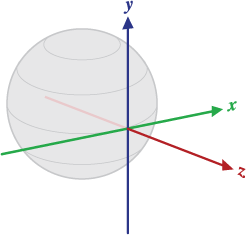
\includegraphics[scale=1]{Gambar/axis-globe.png}
	\caption{Sistem koordinat sensor rotasi vektor terhadap Bumi} 
	\label{fig:axis-globe}
	\end{figure}
	\item values[0]: \(x \sin (\frac{\theta}{2})\)
	\item values[1]: \(y \sin (\frac{\theta}{2})\)
	\item values[2]: \(z \sin (\frac{\theta}{2})\)
	\item values[3]: \(\cos (\frac{\theta}{2})\)
	\item values[4]: Perkiraan akurasi (dalam radian) (-1 jika tidak tersedia) 
\end{itemize}



\end{itemize}


\section{Google VR SDK}
\label{sec:google_vr_sdk}
Google VR SDK digunakan untuk membantu dalam pembuatan aplikasi Virtual Reality pada \textit{smartphone}.\cite{google_vr_developers} Google VR SDK memberikan beberapa fitur sebagai berikut :
\begin{itemize}
	\item \textbf{Binocular rendering}: Fitur untuk tampilan layar terpisah untuk masing-masing dalam pandangan VR.
	\item \textbf{Spatial audio}: Fitur untuk mengeluarkan suara yang datang dari daerah-daerah tertentu dari dunia VR.
	\item \textbf{Head movement tracking}: Fitur untuk mendapatkan memperbaharui penglihatan dunia VR yang sesuai dengan gerakan kepala pengguna.
	\item \textbf{Trigger input}: Fitur untuk memberikan masukan pada dunia VR dengan menekan tombol.
\end{itemize}

Ada beberapa persyaratan untuk menggunakan Google VR SDK, persyaratan tersebut adalah:
\begin{itemize}
	\item Android Studio versi 1.0 atau lebih.
	\item Android SDK versi 23
	\item Gradle versi 23.0.1 atau lebih. Android Studio akan membantu meningkatkan versinya jika versinya terlalu rendah.
	\item Perangkat Android fisik yang menjalankan Android versi 4.4 (KitKat) atau lebih.
\end{itemize}

Dalam membuat aplikasi Google Cardboard VR membutuhkan beberapa API(Application Program Interface) dari Google VR SDK. API-API umum yang akan digunakan adalah sebagai berikut. 
\begin{itemize}
	\item API audio: API untuk membuat implementasi dari \textbf{\textit{Spatial Audio}} (Metode untuk memberikan sumber suara yang sesuai dengan tempatnya dalam ruang tiga dimensi).
	\item API base: API untuk fondasi dari suatu aplikasi Google VR.
\end{itemize}

\subsection{API Audio}
\label{sec:api_audio}

API ini membantu developer untuk memberikan sumber suara secara spasial dalam tiga dimensi, termasuk jarak dengan tinggi isyarat sumber suara.\cite{google_vr_developers} Pada API ini hanya terdapat satu class utama yaitu \textbf{GvrAudioEngine}. \textbf{GvrAudioEngine} mampu memutarkan suara secara spasial dalam dua cara yang berbeda :
\begin{itemize}
	\item Metode pertama dikenal sebagai \textit{Sound Object rendering}. Metode ini memungkinkan pengguna membuat sumber suara virtual dalam ruang tiga dimensi.
	\item Metode kedua memungkinkan pengguna untuk memutar kembali rekaman \textit{Ambisonic soundfield}. Rekaman \textit{Ambisonic soundfield} adalah file audio spasial \textit{multi-channel}.
\end{itemize}
API ini juga dapat memutarkan suara secara \textit{stereo}. Kelas \textbf{GvrAudioEngine} memiliki tiga buah \textit{nested class} yaitu:
\begin{itemize}
	\item GvrAudioEngine.DistanceRolloffModel: Kelas ini mendefinisikan konstanta-konstanta yang mewakili perbedaan jarak dari efek model-model \textit{rolloff}. 
	\item GvrAudioEngine.MaterialName: Kelas ini mendefinisikan konstanta-konstanta yang mewakili bahan permukaan ruangan untuk disesuaikan dengan efek suara pada suatu ruangan.
	\item GvrAudioEngine.RenderingMode: Kelas ini mendefinisikan konstanta-konstanta untuk menyesuaikan dengan mode \textit{rendering}. Semakin baik kualitas \textit{rendering} akan semakin besar penggunaan CPU(Central Processing Unit).
\end{itemize}

\subsection{API Base}
\label{sec:api_base}

API ini digunakan sebagai fondasi dari suatu aplikasi Google VR.\cite{google_vr_developers} Fitur-fitur \textit{Binocular rendering, Head movement tracking,} dan \textit{Trigger input} diberikan pada API ini. Kelas-kelas penting yang ada di API ini adalah AndroidCompat, Eye, GvrActivity, GvrView, HeadTransform, Viewport.
\begin{itemize}
	\item AndroidCompat\\
Kelas ini merupakan kelas utilitas untuk menggunakan fitur VR. Fitur-fitur ini mungkin tidak tersedia pada semua versi android. Kelas ini memiliki \textit{method}-\textit{method} sebagai berikut:
\begin{itemize}
	\item setSustainedPerformanceMode(Activity activity, boolean enabled): \\
	Method ini digunakan untuk mengubah window android ke mode performa secara berkelanjutan.
	\item public static void setVrModeEnabled (Activity activity, boolean enabled): \\
	Mengatur pengaturan yang tepat untuk "mode VR" pada suatu Activity. Method ini tidak digunakan karena hanya dapat digunakan pada Android N+.
	\item public static boolean trySetVrModeEnabled (Activity activity, boolean enabled): 
	Method ini kegunaanya sama dengan \textit{method} \textbf{setVrModeEnabled (Activity activity, boolean enabled)}, namun mengembalikan boolean true jika berhasil dan sebaliknya.
\end{itemize}
	\item Eye\\
Kelas ini mendefinisikan detail pe-\textit{render}-an stereoskopik mata. Stereoskopik adalah sebuah teknik untuk membuat atau menampilkan ilusi mendalam pada sebuah gambar untuk penglihatan binokular. Method penting yang dimiliki kelas ini adalah \textbf{public float[] getEyeView ()}. Method ini mengembalikan matriks yang mengubah kamera virtual ke mata. Transformasi yang diberikan termasuk melacak rotasi kepala, perubahan posisi dan perubahan IPD(interpupillary distance).
	\item GvrActivity\\
Kelas ini merupakan Activity dasar yang menyediakan integrasi yang mudah dengan headset Google VR. Kelas ini mengekspos kejadian untuk berinteraksi dengan headset Google VR dan menangani detail-detail yang biasa diperlukan saat membuat suatu Activity untuk pe-\textit{render}-an VR. Activity ini membuat layar tetap menyala selama perangkat android bergerak. Jika tidak ada pergerakan dari perangkat android maka layar reguler (\textit{wakeclock}) akan ditampilkan. Pada kelas ini terdapat \textit{method} \textbf{onCardboardTrigger ()} untuk mendeteksi ketika Cardboard Trigger sedang ditarik dan dilepaskan (Magnet yang berada pada sisi Google Cardboard).
	\item GvrView\\
	Kelas ini merupakan kelas View yang menyediakan pe-\textit{render}-an VR. Kelas ini didesain untuk berkerja pada mode layar penuh dengan orientasi \textit{landscape} atau \textit{reverse landscape}. Kelas View ini dapat digunakan dengan mengimplements salah satu Interface pe-\textit{render}-an. Interface-interface tersebut adalah:
	\begin{itemize}
		\item GvrView.StereoRenderer: Interface untuk pe-\textit{render}-an detail stereoskopik secara abstrak oleh pe-\textit{render}-an.
		\item GvrView.Renderer: Interface untuk mesin yang kompleks yang membutuhkan untuk menangai semua detail pe-\textit{render}-an.
	\end{itemize}
Kelas GvrView.Renderer jarang digunakan dan sebaiknya tidak digunakan jika tidak sangat dibutuhkan.
Ketika suatu kelas mengimplement Kelas GvrView.StereoRenderer, kelas tersebut harus melakukan implementasi \textit{method}-\textit{method} berikut ini:
\begin{itemize}
	\item \textbf{public void onNewFrame(HeadTransform headTransform)}\\
	\textit{method} ini terpanggil ketika Framebaru akan digambar. Method ini memungkinkan untuk membedakan antara pe-\textit{render}-an pandangan mata dan frame-frame yang berbeda. Setiap operasi per-frame harus tidak spesifik pada satu tampilan saja.
	\item \textbf{public abstract void onDrawEye (Eye eye)}\\
	Method ini meminta untuk menggambar suatu konten dari sudut pandang mata.
	\item \textbf{public abstract void onFinishFrame (Viewport viewport)}\\
	Method ini dipanggil ketika suatu frame telah selesai. Dengan pemanggilan ini, konten frame telah di gambar dan jika koreksi distorsi diaktifkan, koreksi \textit{}distrosi akan diterapkan. Setiap pe-\textit{render}-an pada tahap ini relatif terhadap seluruh permukaan, tidak terhadap satu pandangan mata tunggal. 
	\item \textbf{public abstract void onRendererShutdown ()}\\
	Method ini dipanggil ketika thread pe-\textit{render}-an sedang menutup. Melepaskan sumber GL(Graphics Library) dan sedang melakukan penutupan operasi pada thread pe-\textit{render}-an. Dipanggil hanya jika sebelumnya ada pemanggilan \textit{method} onSurfaceCreated.
	\item \textbf{public abstract void onSurfaceChanged (int width, int height)}\\
	Dipanggil ketika ada perubahan dimensi permukaan. Semua nilai adalah relatif ke ukuran yang dibutuhkan untuk me-\textit{render} sebuah mata.
	\item \textbf{public abstract void onSurfaceCreated (EGLConfig config)}\\
	Method ini dipanggil ketika suatu permukaan dibangun atau dibangun ulang.
\end{itemize}
\item HeadTransform\\
	Method ini mendeskripsikan transformasi kepala secara \textit{independent} dari setiap parameter mata. Kelas ini digunakan di kelas GvrView.StereoRenderer sebagai parameter pada \textit{method} \textbf{onNewFrame}. Method-method yang perlu diperhatikan pada kelas ini adalah:
	\begin{itemize}
		\item \textbf{public void getHeadView (float[] headView, int offset)}\\
		Method ini digunakan untuk mendapatkan matriks transformasi dari kamera virtual ke kepala. Kepala di sini diartikan sebagai titik tengah diantara kedua mata. Matriks yang didapatkan akan disimpan pada parameter \textbf{headView}.
		\item \textbf{public void getQuaternion (float[] quaternion, int offset)}\\
		Method ini digunakan untuk mendapatkan kuaternion yang menjadi representasi dari rotasi kepala.
	\end{itemize}
	\item Viewport\\
	Kelas ini diartikan sebagai \textit{viewport}(area pandang) berbentuk persegi.
\end{itemize}
\section{Teori Kuaternion}
\label{sec:teori_quaternion}

Pada Android SDK \textbf{SensorEvent.values}  tipe sensor \textbf{Sensor.TYPE\_ROTATION\_VECTOR}, yaitu tipe sensor yang mendeteksi vektor perputaran pada \textit{smartphone}.\cite{android_developers} Tipe sensor ini dijelaskan akan mengembalikan nilai-nilai dari komponen kuaternion. 
Kuaternion adalah objek penggabungan dari suatu skalar dengan suatu vektor, sesuatu yang tidak dapat diartikan dalam aljabar linear biasa.\cite{kuipers:1999} Kuaternion ditemukan oleh William Rowan Hamilton dengan memperpanjang notasi dari bilangan kompleks menjadi Kuaternion. 
\subsection{Struktur Ajabar}
Karena Kuaternion merupakan bilangan kompleks yang diperpanjang notasinya, struktur aljabar Kuaternion hampir mirip dengan bilangan kompleks. Untuk mengerti struktur-struktur aljabar kuaternion, diperlukan untuk mengerti  bilangan kompleks terlebih dahulu. Berikut adalah penjelasan singkat tentang bilangan kompleks. 


\subsubsection{Bilangan Kompleks}
\label{sssec:bilangan_kompleks}
\cite{kuipers:1999}
Bilangan kompleks adalah bilangan yang merupakan gabungan dari bilangan imajiner dengan bilangan riil. Notasi umum dari bilangan kompleks adalah :

\begin{equation}
	a+bi
\label{eq:notasi_umum_bilangan_kompleks}
\end{equation}
Pada notasi \ref{eq:notasi_umum_bilangan_kompleks} bilangan \(a\) dengan \(b\) merupakan bilangan riil, dan \(i\) merupakan bilangan imajiner tertentu yang memiliki sifat \(i^2=-1\). Bilangan kompleks juga dapat beroperasi dengan bilangan kompleks lainnya seperti penjumlahan, perkalian, pengurangan, dan pembagian. Berikut adalah contoh-contoh operasi pada bilangan kompleks \ref{eq:notasi_umum_bilangan_kompleks} dengan bilangan kompleks \(c+di\):
\begin{itemize}
	\item Penjumlahan\\
	\[
	 (a + bi) + (c + di) = (a+c) + i(b+d)
	\]
	\item Perkalian\\
	\[
	 (a + bi)(c + di) = (ac−bd) + (bc+ad)i
	\]
	\item Pengurangan\\
	\[
	 (a + bi) - (c + di) = (a-c) + i(b-d)
	\]
	\item Pembagian\\
	\[
	 \frac{(a + bi)}{(c + di)} = \frac{(ac+bd)}{c^2+d^2} + i \frac{bc-ad}{c^2+d^2}
	\]
\end{itemize}
Pada operasi jumlah dan kali untuk kedua bilangan kompleks tersebut memiliki hukum assosiatif dan komutatif. Notasi \ref{eq:penjumlahan_hukum} menunjukkan bagaimana bagaimana kedua hukum tersebut berlaku pada operasi jumlah.
\begin{equation}
	\begin{split}
	(a+ib) + (c+id) = (a+c) + i(b+d)=\\
	(c+id) + (a+ib) = (c+a) + i(d+b)
	\end{split}
\label{eq:penjumlahan_hukum}
\end{equation}

Suatu bilangan dapat dikatakan konjugasi kompleks dari suatu bilangan kompleks jika nilai bilangan riilnya sama, tetapi nilai bilangan imajinernya berlawanan dengan nilai pada bilangan kompleks tersebut. Maka konjugasi kompleks dari bilangan kompleks \ref{eq:notasi_umum_bilangan_kompleks} adalah \(a-bi\). 

Bilangan kompleks ini dapat digunakan untuk rotasi vektor pada bidang dua dimensi. Rotasi ini dapat dilakukan dengan mengalikan suatu vektor dengan bilangan imajiner $i$. Mengalikan suatu vektor dengan bilangan imajiner $i$ akan memutar vektor sebesar $90^{\circ}$ berlawanan arah jarum jam. Mengalikan suatu vektor dengan bilangan imajiner $i^2$ akan memutar vektor sebesar $180^{\circ}$ berlawanan arah jarum jam. Untuk memperjelas perputaran dengan bilangan kompleks diberikan contoh berikut:
Sebuah vektor $v = 3 + i3$ akan diputar $90^{\circ}$ berlawanan arah jarum jam dengan mengalikan vektor tersebut dengan bilangan imajiner $i$. Maka vektor hasil perputarannya($v'$) adalah :
\begin{equation}
	\begin{split}
		v' = &i(3 + i3)\\
		= & i3 + i^2 3\\
		= & i3 + (-1) 3\\
		= & -3 + i3
	\end{split}
\label{eq:rotasi_kompleks}
\end{equation}
\begin{figure}[htbp]
\centering
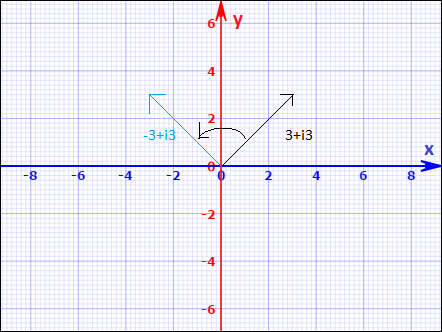
\includegraphics[scale=1]{Gambar/diagram-rotasi-kompleks.PNG}
\caption{Contoh perputaran dengan bilangan kompleks} 
\label{fig:diagram-rotasi-kompleks}
\end{figure}
Dengan bilangan pada bilangan riil diasumsikan sebagai nilai pada sumbu x dan bilangan yang dikalikan dengan bilangan $i$ diasumsikan pada sumbu y($x + iy$) Seperti yang ditunjukkan pada Gambar \ref{fig:diagram-rotasi-kompleks}. Oleh karena itu rumus perputaran menggunakan bilangan kompleks dapat di rumuskan sebagai berikut: 
\[
	v' = v\times(\cos \theta + i \sin \theta)
\]
dengan $\theta$ adalah besar sudut perputaran. Jika vektor $v = 3 + i3$ diputar $30^{\circ}$ berlawanan arah jarum jam menggunakan konsep diatas, akan menghasilkan vektor berikut:

\begin{equation}
	\begin{split}
		v' = &(3 + i3)(\cos 30^{\circ} + i \sin 30^{\circ})\\
		= & (3 + i3)(\frac{\sqrt{3}}{2} + i \frac{1}{2})\\
		= & \frac{3\sqrt{3}-3}{2} + i\frac{3\sqrt{3}+3}{2}\\
		= & 1.098 + i4.098
	\end{split}
\label{eq:rotasi_kompleks_tiga_puluh_derajat}
\end{equation}

Dari persamaan tersebut dapat digambarkan pada Gambar \ref{fig:diagram-rotasi-kompleks1}.

\begin{figure}[htbp]
\centering
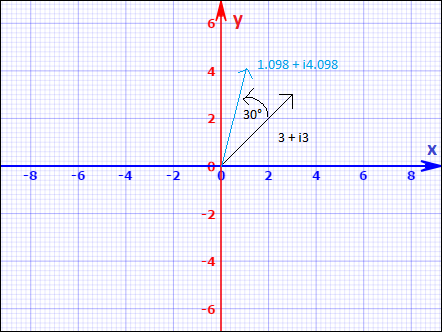
\includegraphics[scale=1]{Gambar/diagram-rotasi-kompleks1.PNG}
\caption{Contoh perputaran tiga puluh derajat dengan bilangan kompleks} 
\label{fig:diagram-rotasi-kompleks1}
\end{figure}
\subsection{\textit{Aljabar Kuaternion} dan Operasi-operasi pada Kuaternion}

Kuaternion ditemukan oleh ahli matematika dan astronomi Inggris, William Rowan Hamilton, dengan memperpanjang aritmetika dari bilangan kompleks.\cite{kuipers:1999} Dari penemuan tersebut William Rowan Hamilton menemukan bahwa dia tidak hanya membutuhkan bilangan imajiner \(i\) saja untuk melakukan rotasi pada ruang tiga dimensi. Dia menemukan bahwa dia juga membutuhkan tiga komponen imajiner lainnya yaitu \(i,j\) dan \(k\). Persamaan umum Kuaternion memiliki empat bilangan riil atau skalar. Persamaan tersebut adalah 

\begin{equation}
	q = q_0 + i q_1 + j q_2 + k q_3	
\label{eq:notasi_kuaternion}
\end{equation}
Ketiga komponen tersebut memiliki relasi sebagai berikut:
\[
	i^2 = j^2 = k^2 = ijk = -1
\]

Hasil dari perkalian dua \textit{kuaternion} memiliki aturan yang lebih rumit, sehingga memiliki aturan-aturan khusus. Berikut aturan-aturan khususnya :
\begin{equation}
	\begin{split}
	& ij = k = -ji\\
	& jk = i = -kj\\
	& ki = j = -ik	
	\end{split}
\label{eq:persamaan_khusus_aturan_quaternion}
\end{equation}\\
Ketiga persamaan di atas mirip dengan aturan tangan kanan (\textit{right-hand rule})pada perkalian cross product dari suatu vektor. Pada Gambar \ref{fig:right-hand-rule}, \(A\) berperan sebagai \(i\), \(B\) berperan sebagai \(j\), dan \(C\) berperan sebagai \(k\).\\
\begin{figure}[htbp]
\centering
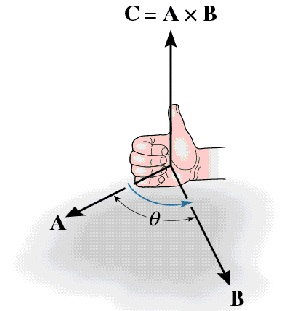
\includegraphics[scale=1]{Gambar/right-hand-rule}
\caption{Right-hand rule dalam \textit{cross product} vektor} 
\label{fig:right-hand-rule}
\end{figure}\\

Seperti pada bilangan kompleks, kuaternion juga memiliki konjugasinya. Konjugasi kuaternion ini akan digunakan untuk melakukan operasi rotasi tiga dimensi(Akan dijelaskan pada subbab Operasi pada Kuaternion). Sama dengan konjugasi pada bilangan kompleks, kuaternion yang bilangan riilnya sama, dan bilangan imajinernya berlawanan dengan kuaternionnya disebut dengan konjugasi kuaternion. Oleh karena itu konjugasi kuaternion dari notasi kuaternion \ref{eq:notasi_kuaternion} adalah: 
\[
	q = q_0 - i q_1 - j q_2 - k q_3
\]
\subsubsection{Operasi pada Kuaternion}
\label{sssec:operasi_pada_kuaternion}
Dua buah kuaternion dapat dikatakan identik jika dan hanya jika kedua kuaternion memiliki komponen yang identik.
\[
	p = p_0 + +ip_1+jp_2+kp_3
\]
dan,
\[
	q = q_0 + i q_1 + j q_2 + k q_3
\]
maka p = q jika dan hanya jika
\begin{equation}
	\begin{split}
	p_0=q_0\\
	p_1=q_1\\
	p_2=q_2\\
	p_3=q_3\\
	\end{split}
\end{equation}
Penjumlahan dari kedua kuaternion di atas dapat diartikan sebagai komponen penjumlahan yaitu:
\[
	(p+q)=(p_0+q_0)+i(p_1+q_1)+j(p_2+q_2)+k(p_3+q_3)
\]
Peralihan dari kedua kuaternion di atas dapat diartikan sebagai komponen perkalian yaitu:
\[
	pq = (p_0 +ip_1+jp_2+kp_3)(q_0 + i q_1 + j q_2 + k q_3)
\]
Begitu pula untuk komponen pengurangan dengan pembagian. 
Dari keempat operasi kuaternion tersebut, operasi kuaternion yang digunakan untuk rotasi bidang tiga dimensi adalah operasi perkalian. Fungsi rotasi vektor dapat menggunakan operasi kuaternion seperti pada bilangan kompleks, dengan rumus:
\[
	v' = qvq^*
\]
dengan,
\begin{itemize}
	\item \(v = 1 + x_v i +y_v j + z_v k\)
	\item \(q = q_0 + i q_1 + j q_2 + k q_3	\)
	\item \(q^* =  q_0 - i q_1 - j q_2 - k q_3\)
	\item \(v' = 1 + x_{v'} i +y_{v'} j + z_{v'} k\)
\end{itemize}
Seperti pada bilangan kompleks, bilangan $q_0 ,i q_1,j q_2,k q_3$ akan memiliki nilai sebagai berikut jika suatu kuaternion ingin digunakan untuk rotasi tiga dimensi:
\begin{equation}
	\begin{split}
	q_0=& \cos (\frac{\theta}{2})\\
	q_1=& \sin (\frac{\theta}{2}) x_f\\
	q_2=& \sin (\frac{\theta}{2}) y_f\\
	q_3=& \sin (\frac{\theta}{2}) z_f\\
	\end{split}
\end{equation}
dengan vektor f ($x_f,y_f,z_f$) merupakan sumbu perputaran dan $\theta$ merupakan besar sudut putar berlawanan arah dengan jarum jam.

\section{Unity Game Engine}
\label{sec:unity_game_engine}

Unity merupakan salah satu \textit{Game Engine} dalam pembuatan permainan dua dimensi atau tiga dimensi.\cite{unity} Unity merupakan \textit{Game Engine} \textit{multi-platform} sehingga permainan yang dibuat menggunakan Unity akan dapat berjalan di berbagai macam perangkat seperti \textit{smartphone}, komputer, \textit{console}, dan lain-lain.  \textit{Game Engine} ini menggunakan bahasa C\# atau Javascript.

Game Engine ini dapat diperoleh secara gratis, yaitu dengan menggunakan Unity Personal Edition. Game Engine edisi Personal ini tidak akan berlaku jika penggunaan unity mendapatkan pendapatan kotor tahunan sebesar USD 100.000. Jika pendapatan kotor tahunan sudah melebihi USD 100.000, pengguna unity personal harus segera mengganti edisi Unity menjadi Unity Plus, Unity Pro, atau Unity Enterprise. Jika menggunakan Unity Personal, \textit{splashscreen} dan logo \textit{icon} pada permainan yang dibuat tidak diganti maupun dihapus. 


 \subsection{Struktur Hierarki GameObject}
 \label{ssec:struktur_hierarki_gameobject}
 
 Hierarki pada unity merupakan kumpulan dari GameObject. \cite{unity_manual} GameObject akan dijelaskan lebih lanjut pada subbab \ref{ssec:gameobject}. Beberapa dari GameObject pada hierarki ini merupakan instansi dari file \textit{assets}. Setiap \textit{scene} akan memiliki hierarki masing-masing. Setiap objek yang di tambahkan pada suatu \textit{scene}(dijelaskan pada subbab \ref{ssec:scene}) akan muncul pada hierarki juga.
 
 Pada hierarki ini juga ada konsep \textit{parent-child} objects. Konsep ini digunakan untuk setiap kumpulan object. Setiap objek yang berada paling luar dinamakan "parent object", dan objek-objek  yang berada didalamnya dinamakan "child object". Suatu parent object juga dapat memiliki parent objek(biasa disebut juka "nested parent object". Contoh dari konsep \textit{parent-child} ada pada Gambar \ref{fig:contoh-hierarchy-parenting}.
 
 
\begin{figure}[htbp]
\centering
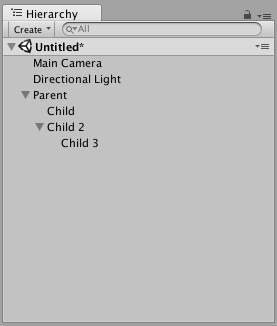
\includegraphics[scale=0.7]{Gambar/hierarchy-parenting.png}
\caption{Contoh Hierarchy Parenting.} 
\label{fig:contoh-hierarchy-parenting}
\end{figure}

\subsection{Prefabs}
\label{ssec:prefabs}

Unity memiliki suatu jenis assets yang dinamakan Prefab. Prefab ini adalah suatu GameObject yang disimpan menjadi assets. Prefab berperan sebagai contoh/\textit{blueprint} dari suatu GameObject. Prefab ini juga dapat dibentuk dari GameObject yang telah dibuat dan menjadi assets, sehingga dapat digunakan pada proyek lain. Prefab juga data di ubah dan dimodif sehingga menjadi sesuai dengan yang diinginkan. 

Dalam membuat Prefab dapat dengan mudah me-\textit{drag and drop} suatu GameObject pada tab Scene ke tab Assets. Begitupula dengan sebaliknya, untuk menggunakan suatu prefab, dapat dengan mudah me-\textit{drag and drop} dari tab Assets ke tab Scene. 

\subsection{Scene}
\label{ssec:scene}

\textit{Scene} menyimpan seluruh objek pada game yang akan dibuat. \textit{Scene} dapat digunakan untuk membuat \textit{main menu, game level}, dan lain sebagainya. Untuk setiap \textit{scene}, akan ditempatkan barang, bangunan, dekorasi, dan lain sebagainya untuk merancang dan membangun suatu permainan bagian per bagian.  

Pada saat pembuatan proyek pertama, unity akan membuatkan suatu \textit{scene} baru. \textit{Scene} tersebut merupakan \textit{scene default}. \textit{Scene} tersebut hanya akan diberikan objek-objek \textit{default} saja seperti kamera dan cahaya. Kamera yang akan diberikan antara dua buah jenis yaitu \textit{orthographic camera} atau \textit{perspective camera}, proyek 2D akan diberikan \textit{orthographic camera} dan proyek 3D akan diberikan \textit{perspective camera}. Contoh dari \textit{scene} default pada proyek 3D ditunjukkan pada Gambar \ref{fig:contoh-scene-kosong}.
 
\begin{figure}[htbp]
\centering
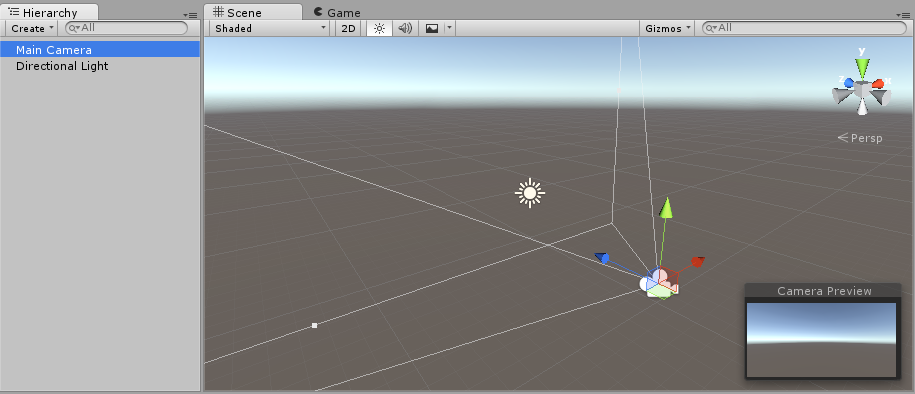
\includegraphics[scale=0.5]{Gambar/new-empty-scene.png}
\caption{Contoh \textit{scene} kosong.} 
\label{fig:contoh-scene-kosong}
\end{figure}


\subsection{GameObject}
\label{ssec:gameobject}
GameObject pada unity yang merupakan representasi karakter, barang, dan pemandangan. GameObject tidak dapat melakukan apa pun dengan sendirinya, tetapi GameObject melakukan sesuatu sesuai dengan komponen yang ada pada GameObject. Komponen menjalankan fungsi-fungsi nyata pada GameObject. Contohnya objek cahaya dapat terbuat dengan menambahkan komponen Light kepada suatu GameObject (Gambar \ref{fig:contoh-component-pada-game-object}).

\begin{figure}[htbp]
\centering
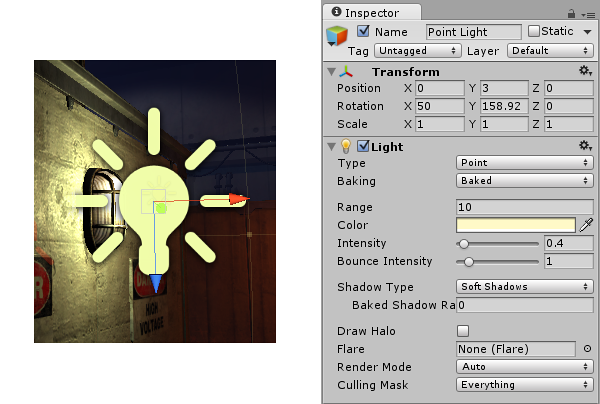
\includegraphics[scale=0.7]{Gambar/contoh-component-pada-game-object.png}
\caption{Contoh penggunaan komponen pada GameObject.} 
\label{fig:contoh-component-pada-game-object}
\end{figure}
 
Selain itu ada pula contoh GameObject Kubus. GameObject ini memiliki komponen Cube(Mesh Filter) dan Mesh Renderer. Kedua komponen tersebut berguna untuk menggambar permukaan dari kubus tersebut. Selain itu ada juga komponen Box Collider yang digunakan untuk menggambarkan \textit{GameObject} tersebut dalam hal-hal fisika seperti gravitasi, gaya, dan lain sebagainya(Gambar \ref{fig:contoh-component-pada-game-object2}).


\begin{figure}[htbp]
\centering
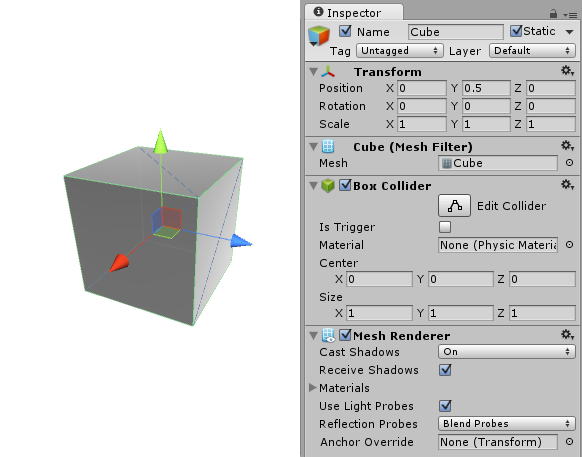
\includegraphics[scale=0.7]{Gambar/contoh-component-pada-game-object2.png}
\caption{Contoh komponen pada GameObject kubus.} 
\label{fig:contoh-component-pada-game-object2}
\end{figure}
 
\subsection{Scripting}

Pembuatan permainan pada Game Engine Unity membutuhkan \textit{script} untuk memberikan logika permainan (\textit{Game Logic}). Pembuatan \textit{script} dapat dilakukan dengan membuat suatu kelas yang merupakan turunan kelas MonoBehavior agar dapat berjalan sesuai dengan sistem internal Unity. \textit{Script} pada Unity bersifat seperti blueprint, sehingga \textit{script} tidak akan dijalankan hingga \textit{script} tersebut dihubungkan dengan suatu GameObject. Menghubungkan \textit{script} dengan GameObject dapat dilakukan dengan menambahkan sebuah Component \textit{Scripts} seperti yang ditunjukkan pada Gambar \ref{fig:contoh-component-scripts}.

\begin{figure}[htbp]
\centering
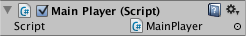
\includegraphics[scale=1]{Gambar/ScriptInInspector.png}
\caption{Contoh Component \textit{script}.} 
\label{fig:contoh-component-scripts}
\end{figure}

Dalam \textit{scripting} pada Unity, ada sejumlah \textit{method} yang akan dieksekusi dalam urutan yang telah ditentukan. Pada skripsi ini hanya akan dijelaskan fungsi-fungsi yang penting saja, untuk penjelasan lebih detail dijelaskan pada alamat web "Unity - Manual" \footnote{https://docs.unity3d.com/Manual/class-ScriptExecution.html}. Perintah-perintah eksekusi ini dijelaskan di bawah ini:
\begin{itemize}
    \item \textbf{Ketika Pertama Kali Scene Dimuat}\\
    \begin{itemize}
        \item Awake:\\
        Fungsi ini selalu dipanggil sebelum fungsi Start dan juga tepat setelah prefab di instansiasikan. (Jika GameObject tidak aktif saat aplikasi baru dimulai, fungsi Awake tidak dipanggil, sampai GameObject diaktifkan).
        \item OnEnable:\\
        Fungsi ini dipanggil sesaat setelah objek diaktifkan. Hal ini terjadi ketika contoh MonoBehaviour dibuat, seperti saat level/scene dimuat atau GameObject dengan komponen \textit{script} di instansiasikan.
    \end{itemize}
    \item \textbf{Sebelum Frame Pertama Dimuat}
    \begin{itemize}
        \item Start:\\
        Fungsi ini  dipanggil sebelum frame pertama dimuat. Untuk setiap objek yang ditambahkan ke \textit{scene}, fungsi Start akan dipanggil pada semua \textit{script} sebelum fungsi Update dipanggil.
    \end{itemize}
    \item \textbf{Urutan Pemanggilan Update}\\
    \begin{itemize}
        \item FixedUpdate:\\
        FixedUpdate akan lebih sering dipanggil dibandingkan dengan fungsi Update. Fungsi ini dapat terpanggil beberapa kali pada suatu \textit{frame} jika \textit{frame rate} rendah. Pada saat \textit{frame rate} tinggi fungsi ini akan selalu terpanggil minimal satu kali setiap frame. Fungsi ini biasanya digunakan untuk melakukan implementasi perhitungan-perhitungan fisika pada permainan. 
        \item Update:\\
        Fungsi Update akan dipanggil di setiap \textit{frame}. Fungsi ini merupakan fungsi inti untuk pergantian pada frame.
        \item LateUpdate:\\
        LateUpdate dipanggil di setiap \textit{frame}, setelah pemanggilan fungsi Update. Semua perhitungan pada Update dipastikan telah dieksekusi pada saat fungsi ini dipanggil. Fungsi ini biasanya digunakan ketika mengimplementasi \textit{third-person camera}, karena \textit{third-person camera} perlu memastikan kalkulasi pergerakan pemain sudah dieksekusi sebelum menggerakkan kamera tersebut.
    \end{itemize}
    \item \textbf{Ketika Aplikasi Berhenti}
    \begin{itemize}
        \item OnApplicationQuit:\\
        Fungsi ini akan dipanggil ketika Aplikasi berhenti.
        \item OnDisable:\\
        Fungsi ini akan dipanggil ketika suatu tingkah laku(\textit{script}) di non-aktifkan.
    \end{itemize}
    \item Flowchart Siklus Script
    Gambar \ref{fig:flowchart_pemanggilan_fungsi} merupakan flowchart urutan pemanggilan fungsi-fungsi script.
    
    \begin{figure}[htbp]
    \centering
    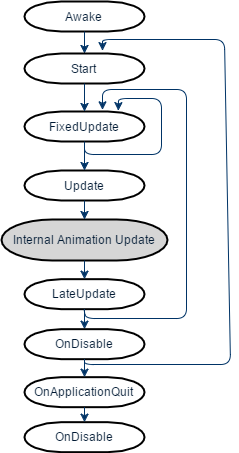
\includegraphics[scale=0.6]{Gambar/unity-script-flowchart.png}
    \caption{Flowchart urutan pemanggilan fungsi-fungsi.} 
    \label{fig:flowchart_pemanggilan_fungsi}
    \end{figure}
    
\end{itemize}
 
 
\subsection{Transformasi Rotasi dan Orientasi}
\label{ssec:transformasi_rotasi_dan_orientasi}

 Setiap GameObject selalu mempunyai komponen Transform untuk memberikan representasi posisi, orientasi, dan skala GameObject tersebut. Komponen ini tidak dapat dihapus. Komponen Transform ini nilainya relatif terhadap nilai komponen Transform pada \textit{parent}-nya. Jika Transform ini tidak memiliki \textit{parent}, nilainya akan relatif pada dunianya (\textit{world space}). 
 
 Komponen Transform memiliki beberapa atribut. Atribut-atribut yang penting pada komponen ini adalah position, lossyScale, dan rotation. Atribut position menyimpan positi dari suatu GameObject. Atribut ini disimpan dengan menggunakan kelas Vector3. Atribut lossyScale menyimpan besar penskalaan suatu GameObject. Atribut lossyScale ini pun disimpan dengan menggunakan kelas Vector3. Atribut rotation digunakan untuk menyimpan orientasi dari suatu GameObject. Atribut rotation berbeda dengan atribut position dan lossyScale. Atribut rotation disimpan dengan menggunakan kelas Quaternion. 
 
 Rotasi pada aplikasi tiga dimensi biasanya menggunakan antara metode Quaternion atau Euler Angles. Masing-masing memiliki kelebihan dan kekurangan. Seperti yang tadi sudah dijelaskan, Unity menggunakan Quaternion dalam memberikan representasi rotasi dan orientasi. Pada kelas Quaternion terdapat atribut yang menyimpan nilai-nilai orientasi pada Euler Angles, sehingga juga unity dapat memberikan representasi rotasi dan orientasi dengan menggunakan Euler Angles.
 
 Kelebihan menggunakan representasi Euler Angles.
 \begin{itemize}
     \item Euler Angles lebih mudah untuk di pahami dalam format tiga sudut pada sumbu-sumbu tiga dimensi.
     \item Euler Angles dapat memberikan representasi rotasi dari satu orientasi ke orientasi dengan sumbu yang lebih besar dari 180 derajat. 
 \end{itemize}
 Kekurangan menggunakan representasi Euler Angles.
 \begin{itemize}
     \item Euler Angles dapat mengalami Gimbal Lock. Gimbal Lock adalah kejadian ketika dua sumbu dari sudut perputaran pada Euler Angles berputar pada poros yang sama.
 \end{itemize}
 
 Kelebihan menggunakan representasi Quaternion.
 \begin{itemize}
     \item Kuaternion tidak mengalami Gimbal Lock.
 \end{itemize}
 Kekurangan menggunakan representasi Quaternion.
 \begin{itemize}
     \item suatu kuaternion tidak dapat memberikan representasi rotasi yang melebihi 180 derajat pada arah mana pun.
     \item Representasi angka-angka pada Quaternion lebih susah untuk dimengerti.
 \end{itemize}
 
 Pada Unity, meski pun semua orientasi disimpan dengan menggunakan Quaternion, tetapi pada \textit{Transform Inspector} (Gambar \ref{}) Unity menampilkan nilai-nilai orientasi pada Euler Angles. Hal ini bertujuan untuk mempermudah mengubah orientasi bagi pengguna, karena nilai-nilainya lebih mudah untuk dimengerti. Representasi pada \textit{Transform Inspector} tersebut menyebabkan masukan yang diberikan oleh pengguna terkadang berbeda dengan data yang disimpan. Contohnya ketika berada pada sudut 365 derajat, maka data yang akan disimpan akan menunjukkan perputaran sebesar 5 derajat saja.
 
 \section{Google VR SDK for Unity}
 \label{sec:google_vr_sdk_for_unity}
 
 Google juga menyediakan SDK untuk \textit{Game Engine} Unity. Berbeda dengan Google Cardboard API, Google VR SDK for Unity tidak hanya berfungsi untuk membuat aplikasi untuk Google Cardboard. Google VR SDK juga berfungsi untuk membuat aplikasi untuk Google Daydream, yaitu Aplikasi VR dari Google sebagai pembaruan Google Cardboard. Google daydream memiliki kelebihan memiliki \textit{remote controller} yang dapat merekam gerakan tangan pengguna. Jadi jika menggunakan Google VR SDK for Unity, pembuat permainan juga dapat membuat pengaturan untuk \textit{remote controller} pada Google Daydream.
 
 Untuk mendapatkan Google VR SDK for Unity, SDK tersebut dapat di download pada halaman situs web Google VR Developers.\cite{google_vr_developers} Pada situs tersebut akan diberikan assets package dengan ekstensi file ".unitypackage". Assets package tersebut akan memasukkan seluruh kebutuhan untuk membuat Google VR pada proyek permainan yang sedang dikerjakan. 
 
 Untuk dapat me-\textit{render} permainan dengan tampilan \textit{stereo rendering} (tampilan layar yang di bagi menjadi dua bagian sesuai dengan mata manusia), hierarki GameObject pada scene yang sedang dikerjakan harus memiliki GvrViewerMain dengan komponen script GvrViewer. GameObject ini dapat diperoleh dengan menggunakan \textit{prefabs} yang telah di-\textit{import}. Selain untuk me-\textit{render}, permainan object tersebut juga melakukan implementasi orientasi pada \textit{smartphone} secara langsung.
 
 Seperti yang sudah dijelaskan Google Cardboard memberikan masukan dengan menarik/menekan pelatuk pada Google Cardboard tersebut. Untuk mendapatkan masukan tersebut, dapat dilakukan dengan cara menggunakan \textit{prefab} GvrEventSystem. Kemudian menambahkan komponen Event Trigger pada GameObject yang akan merespons masukan tersebut. Respons dapat dilakukan dengan menambahkan Script baru pada GameObject tersebut.